\documentclass[12pt,a4paper]{aktu}
\usepackage{times}
\usepackage[T1]{fontenc}
\usepackage{titlesec}
\usepackage{geometry}
\usepackage{setspace}
\usepackage{graphicx}
\usepackage{comment}
\usepackage{tikz}
\usetikzlibrary{shapes.geometric, arrows.meta, positioning}
\usepackage{titlesec, titletoc}
\geometry{total={210mm,297mm},
left=3.5cm,right=2cm,
top=3.5cm,bottom=2 cm}

\usepackage{titletoc}
\providecommand{\normal}{\fontsize{12pt}{16pt}\selectfont}
\providecommand{\size}{\fontsize{14pt}{18pt}\selectfont}
\providecommand{\bigsize}{\fontsize{16pt}{20pt}\selectfont}
\providecommand{\bigbigsize}{\fontsize{20pt}{24pt}\selectfont}
\titleformat{\chapter}[display]
  {\bigbigsize \bfseries \centering}{\MakeUppercase{\chaptertitlename}\ \thechapter}{40pt}{\bigsize\MakeUppercase }
\titlespacing*{\chapter}{-10pt}{-20pt}{40pt}

\titlecontents{chapter}[6em]{\bigskip\bfseries}%\vspace{1cm}%
{\contentslabel[\MakeUppercase{\chaptername}~\thecontentslabel]{7em}\MakeUppercase}{\MakeUppercase}%numberless chapters%
{\hfill\contentspage}[\medskip]%
 \titleformat{\section}
{\normalfont\size\bfseries}{\thesection}{1em}{}
\titleformat{\subsection}
{\normalfont\normalsize\bfseries}{\thesubsection}{1em}{}
\titleformat{\subsubsection}
{\normalfont\normalsize\bfseries\textit}{\thesubsubsection}{1em}{}
\titleformat{\paragraph}[runin]
{\normalfont\normalsize\bfseries}{\theparagraph}{1em}{}
\titleformat{\subparagraph}[runin]
{\normalfont\normalsize\bfseries}{\thesubparagraph}{1em}{}
\titleformat{name=\section,numberless}
{\filcenter\Large\bfseries}
{}
{.5em}
{}   
\begin{document}
%\doublespacing
\setstretch{1.5}
\pagenumbering{roman}
% !TEX root = ../main.tex
\bgroup
\catcode`@=11
\gdef\getfontsize{\f@size pt}
\egroup
\providecommand{\normal}{\fontsize{12pt}{16pt}\selectfont}
\providecommand{\size}{\fontsize{14pt}{18pt}\selectfont}
\providecommand{\bigsize}{\fontsize{16pt}{20pt}\selectfont}
\providecommand{\bigbigsize}{\fontsize{20pt}{24pt}\selectfont}
\title{\bigbigsize \textbf{MEV Aware DeFi Liquidation System}}


% If you wish to list your previous degrees on the cover page, use the 
% previous degrees command:
%       \prevdegrees{A.A., Harvard University (1985)}
% You can use the \\ command to list multiple previous degrees
%       \prevdegrees{B.S., University of California (1978) \\
%                    S.M., Massachusetts Institute of Technology (1981)}
%%%%%\supervisor{Dr. Vaibhav Vyas}{Associate Professor}

% This is the department committee chairman, not the thesis committee
% chairman.  You should replace this with your Department's Committee
% Chairman.
%\chairman{Arthur C. Chairman}{Chairman, Department Committee on Graduate Theses}

% Make the titlepage based on the above information.  If you need
% something special and can't use the standard form, you can specify
% the exact text of the titlepage yourself.  Put it in a titlepage
% environment and leave blank lines where you want vertical space.
% The spaces will be adjusted to fill the entire page.  The dotted
% lines for the signatures are made with the \signature command.
\thispagestyle{empty}
\maketitle
\restoregeometry
\newpage


\clearpage
% !TEX root = ../main.tex
\providecommand{\normal}{\fontsize{12pt}{16pt}\selectfont}
\providecommand{\size}{\fontsize{14pt}{18pt}\selectfont}
\providecommand{\bigsize}{\fontsize{16pt}{20pt}\selectfont}
\providecommand{\bigbigsize}{\fontsize{20pt}{24pt}\selectfont}
\begin{center}
{\size\textbf{VISION AND MISSION}}
\end{center}
\vspace{5mm}

\noindent\textbf{VISION OF THE INSTITUTE}

\vspace{2mm}
JSS Academy of Technical Education Noida aims to become an Institution of excellence in imparting quality Outcome Based Education that empowers the young generation with Knowledge, Skills, Research, Aptitude and Ethical values to solve Contemporary Challenging Problems.

\vspace{5mm}
\noindent\textbf{MISSION OF THE INSTITUTE}
\begin{enumerate}
    \item Develop a platform for achieving globally acceptable level of intellectual acumen and technological competence.
\item Create an inspiring ambience that raises the motivation level for conducting quality research.
\item Provide an environment for acquiring ethical values and positive attitude.
\end{enumerate}

\vspace{5mm}
\noindent\textbf{VISION OF THE DEPARTMENT}

\vspace{2mm}
“To spark the imagination of the Computer Science Engineers with values,skills and creativity to solve the real-world problems.”

\vspace{5mm}
\noindent\textbf{MISSION OF THE DEPARTMENT}
\begin{enumerate}
    \item To inculcate creative thinking and problem-solving skills through effective teaching, learning and research.
    \item To empower professionals with core competency in the field of Computer Science and Engineering.
   \item  To foster independent and lifelong learning with ethical and social responsibilities.
\end{enumerate}


\clearpage
% !TEX root = ../main.tex
\providecommand{\normal}{\fontsize{12pt}{16pt}\selectfont}
\providecommand{\size}{\fontsize{14pt}{18pt}\selectfont}
\providecommand{\bigsize}{\fontsize{16pt}{20pt}\selectfont}
\providecommand{\bigbigsize}{\fontsize{20pt}{24pt}\selectfont}
\begin{flushleft}
\size\textbf{PROGRAM OUTCOMES(POs)}
\end{flushleft}

\noindent Engineering Graduates will be able to:

\vspace{3mm}
\noindent\textbf{PO1: Engineering knowledge:} Apply the knowledge of mathematics, science, engineering fundamentals, and an engineering specialization to the solution of complex engineering problems.\\[2mm]
\textbf{PO2: Problem analysis:} Identify,formulate,review research literature,and analyze complex engineering problems reaching substantiated conclusions using first principles of mathematics, natural sciences, and engineering sciences.\\[2mm]
\textbf{PO3: Design/development of solutions:} Design solutions for complex engineering problems and design system components or processes that meet the specified needs with appropriate consideration for the public health and safety, and the cultural, societal, and environmental considerations.\\[2mm]
\textbf{PO4: Conduct investigations of complex problems:} Use research-based knowledge and research methods including design of experiments, analysis and interpretation of data, and synthesis of the information to provide valid conclusions.\\[2mm]
\textbf{PO5: Modern tool usage:} Create, select, and apply appropriate techniques, resources, and modern engineering and IT tools including prediction and modeling to complex engineering activities with an understanding of the limitations.\\[2mm]
\textbf{PO6: The engineer and society:} Apply reasoning informed by the contextual knowledge to assess societal, health, safety, legal and cultural issues and the consequent responsibilities relevant to the professional engineering practice.\\[2mm]
\textbf{PO7: Environment and sustainability:} Understand the impact of the professional engineering solutions in societal and environmental contexts,and demonstrate the knowledge of, and need for sustainable development.\\[2mm]
\textbf{PO8: Ethics:} Apply ethical principles and commit to professional ethics and responsibilities and norms of the engineering practice.\\[2mm]
\textbf{PO9: Individual and teamwork:} Function effectively as an individual,and as a member or leader in diverse teams, and in multidisciplinary settings.\\[2mm]
\textbf{PO10: Communication:} Communicate effectively on complex engineering activities with the engineering community and with society at large, such as, being able to comprehend and write effective reports and design documentation,make effective presentations,and give and receive clear instructions.\\[2mm]
\textbf{PO11: Project management and finance:} Demonstrate knowledge and understanding of the engineering and management principles and apply these to one’s own work,as a member and leader in a team, to manage projects and in multidisciplinary environments.\\[2mm]
\textbf{PO12: Life-long learning:} Recognize the need for,and have the preparation and ability to engage in independent and life-long learning in the broadest context of technological change.

\vspace{5mm}
\noindent\textbf{PROGRAM EDUCATIONAL OUTCOMES (PEOs)}

\vspace{3mm}
\noindent\textbf{PEO1:} To apply computational skills necessary to analyze, formulate and solve engineering problems.\\[2mm]
\textbf{PEO2:} To establish a entrepreneurs,and work in interdisciplinary research and development organizations as an individual or in a team.\\[2mm]
\textbf{PEO3:} To inculcate ethical values and leadership qualities in students to have a successful career.\\[2mm]
\textbf{PEO4:} To develop analytical thinking that helps them to comprehend and solve real-world problems and inherit the attitude of lifelong learning for pursuing higher education.

\vspace{5mm}
\noindent\textbf{PROGRAM SPECIFIC OUTCOMES(PSOs)}

\vspace{3mm}
\noindent\textbf{PSO1:} Acquiring in depth knowledge of theoretical foundations and issues in Computer Science to induce learning abilities for developing computational skills.\\[2mm]
\textbf{PSO2:} Ability to analyse, design, develop, test and manage complex software system and applications using advanced tools and techniques.


\clearpage
% !TEX root = ../main.tex
% Please add the following required packages to your document preamble:
% \usepackage{graphicx}
% \usepackage[table,xcdraw]{xcolor}
% Beamer presentation requires \usepackage{colortbl} instead of \usepackage[table,xcdraw]{xcolor}
\providecommand{\normal}{\fontsize{12pt}{16pt}\selectfont}
\providecommand{\size}{\fontsize{14pt}{18pt}\selectfont}
\providecommand{\bigsize}{\fontsize{16pt}{20pt}\selectfont}
\providecommand{\bigbigsize}{\fontsize{20pt}{24pt}\selectfont}
% Please add the following required packages to your document preamble:
% \usepackage{graphicx}
% \usepackage[table,xcdraw]{xcolor}
% Beamer presentation requires \usepackage{colortbl} instead of \usepackage[table,xcdraw]{xcolor}
%\begin{table}[h!]
\begin{flushleft}
\textbf{\size{Course Outcomes(COs)}}
\end{flushleft}

\noindent\textbf{C410.1:} Identify, formulate, design and analyze a research based/web based problem.\\ 
\textbf{C410.2:} Communicate effectively in verbal and written form\\ 
\textbf{C410.3:} Apply appropriate computing, and engineering skills for obtaining solution to  the formulated problem within a stipulated time.\\
\textbf{C410.4:} Work effectively as a part of team in multi-disciplinary areas.\\ 
\textbf{C410.5:} Consolidate the final outcome in the form of a publication.

\vspace{5mm}
\begin{flushleft}
\size\textbf{CO-PO-PSO Mapping}
\end{flushleft}
% Please add the following required packages to your document preamble:
% \usepackage{graphicx}
% Please add the following required packages to your document preamble:
% \usepackage{graphicx}
% Please add the following required packages to your document preamble:
% \usepackage{graphicx}
% \usepackage[table,xcdraw]{xcolor}
% Beamer presentation requires \usepackage{colortbl} instead of \usepackage[table,xcdraw]{xcolor}
% Please add the following required packages to your document preamble:
% \usepackage{graphicx}
% Please add the following required packages to your document preamble:
% \usepackage{graphicx}
% Please add the following required packages to your document preamble:
% \usepackage{graphicx}
\renewcommand{\arraystretch}{2}

\begin{table}[h!]
\setlength{\tabcolsep}{2.5pt}
\centering
\resizebox{\columnwidth}{!}{%
\begin{tabular}{l|c|c|c|c|c|c|c|c|c|c|c|c|c|c|}
\cline{2-15}
 &
  \multicolumn{1}{l|}{\size\textbf{PO1}} &
  \multicolumn{1}{l|}{\size\textbf{PO2}} &
  \multicolumn{1}{l|}{\size\textbf{PO3}} &
  \multicolumn{1}{l|}{\size\textbf{PO4}} &
  \multicolumn{1}{l|}{\size\textbf{PO5}} &
  \multicolumn{1}{l|}{\size\textbf{PO6}} &
  \multicolumn{1}{l|}{\size\textbf{PO7}} &
  \multicolumn{1}{l|}{\size\textbf{PO8}} &
  \multicolumn{1}{l|}{\size\textbf{PO9}} &
  \multicolumn{1}{l|}{\size\textbf{PO10}} &
  \multicolumn{1}{l|}{\size\textbf{PO11}} &
  \multicolumn{1}{l|}{\size\textbf{PO12}} &
  \multicolumn{1}{l|}{\size\textbf{PSO1}} &
  \multicolumn{1}{l|}{\size\textbf{PSO2}} \\ \hline
  \multicolumn{1}{|l|}{\size\textbf{C410.1}} & 3 & 3 & 3 & 3 & 2 & 3 & 3 & 3 & 3 & 3 & 2 & 3 & 3 & 3 \\ \hline
\multicolumn{1}{|l|}{\size\textbf{C410.2}} & 2 & 2 & 2 & 2 & 2 & 2 & 2 & 2 & 2 & 3 & 2 & 3 & 2 & 3 \\ \hline
\multicolumn{1}{|l|}{\size\textbf{C410.3}} & 3 & 3 & 3 & 3 & 3 & 3 & 2 & 3 & 3 & 3 & 3 & 3 & 3 & 3 \\ \hline
\multicolumn{1}{|l|}{\size\textbf{C410.4}} & 3 & 3 & 3 & 3 & 2 & 3 & 2 & 3 & 3 & 3 & 3 & 3 & 3 & 3 \\ \hline
\multicolumn{1}{|l|}{\size\textbf{C410.5}} & 3 & 3 & 3 & 3 & 3 & 3 & 3 & 3 & 3 & 3 & 3 & 3 & 3 & 3 \\ \hline
\multicolumn{1}{|l|}{\size\textbf{C410}} &
  \size\size\textbf{2.80} &
  \size\textbf{2.80} &
  \size\textbf{2.80} &
 \size \textbf{2.80} &
  \size\textbf{2.40} &
  \size\textbf{2.80} &
  \size\textbf{2.40} &
  \size\textbf{2.80} &
  \size\textbf{2.80} &
 \size \textbf{3.00} &
  \size\textbf{2.60} &
  \size\textbf{3.00} &
  \size\textbf{2.80} &
  \size\textbf{3.00} \\ \hline
\end{tabular}%
}
\end{table}




\clearpage
% !TEX root = ../main.tex
\begin{center}
\addcontentsline{toc}{section}{Declaration}
\chapter*{\size {\textit{\textbf{DECLARATION}}}}   
\end{center}

\doublespacing
\textit{We hereby declare that this synopsis submission is our own work and that, to the best of our knowledge and belief, it contains no material previously published or written by another person nor material which to a substantial extent has been accepted for the award of any other degree or diploma of the university or other institute of higher learning, except where due acknowledgment has been made in the text.}

\vspace{5mm}
\begin{flushleft}
Name : Kashish Gupta\\
Roll. No. : 2300911530066 \\
\vspace{5mm}
(Candidate Signature) \\
\vspace{5mm}
Name : Vertika Singh\\
Roll. No. : 2300911530132\\
\vspace{5mm}
(Candidate Signature) \\
\vspace{5mm}
Name : Avinash Kumar Ankur\\
Roll. No. : 2300911530036\\
\vspace{5mm}
(Candidate Signature) \\
\vspace{5mm}
\vspace{5mm}
\end{flushleft}
\restoregeometry
\newpage
%\newgeometry{top=70mm}
\begin{center}
\addcontentsline{toc}{section}{Certificate}
\chapter*{\size {\textbf{CERTIFICATE}}} 
\end{center}

\doublespacing
This is to certify that project synopsis report entitled “..........................................................\\...................................................................................................................................................”\\which
is submitted by ................................................................................................................. 
\\.................................................................................................................................................... 
in partial fulfillment of the requirement for the award of degree B. Tech. in Department of Computer Science and Engineering-AIML of Dr. APJ Abdul Kalam Technical University, Uttar Pradesh, Lucknow is a record of the candidate’s own work carried out by him/her under my supervision. The matter embodied in this report is original and has not been submitted for the award of any other degree.

\vspace{15 mm}

\begin{flushleft}

Signature\\
\vspace{10 mm}
Name of Supervisor: Ms. Priya Singh\\
Designation: Assistant Professor\\
Address: JSS Academy of Technical Education, Noida\\
\vspace{10mm}
Date:
\end{flushleft}
\restoregeometry
\newpage

\newpage
\begin{abstractpage}
\addcontentsline{toc}{section}{Abstract}
% !TEX root = ../main.tex

Decentralized finance (DeFi) lending protocols rely on automated liquidations to maintain protocol solvency when collateral values fall below defined health thresholds. In public blockchain networks like Ethereum, liquidation calls submitted to the public mempool expose transactions to predatory Maximal Extractable Value (MEV) extraction, such as front-running, sandwich attacks, and priority gas auctions (PGAs). These competitive auctions consume disproportionate network bandwidth, drive up transaction fees, and induce latency that often leads to liquidation failure and bad debt accumulation for protocols.

This project proposes an MEV-Aware DeFi Liquidation System designed to execute undercollateralized debt liquidations efficiently while mitigating negative externalities associated with public mempool competition. The proposed framework integrates private transaction order flows, dynamic auction routing, and predictive health-factor monitoring powered by machine learning algorithms. By analyzing historical mempool dynamics, on-chain volatility, and slippage thresholds, the system schedules and bundles liquidations to bypass public searcher races. The expected outcome is a robust, low-latency liquidation mechanism that minimizes value leakage to searchers, preserves collateral recovery value for borrowers, and enhances protocol solvency across high-volatility market regimes.

\vspace{1.5em}
\noindent\textbf{Keywords:} Decentralized Finance (DeFi), Maximal Extractable Value (MEV), Lending Protocols, Liquidations, Front-running, Solvency, Machine Learning.

\end{abstractpage}
\restoregeometry


\pagestyle{plain}

\doublespacing
% !TEX root = ../main.tex

\newgeometry{top=35mm}

\addcontentsline{toc}{section}{List of Figures}
\renewcommand*\listfigurename{\size\textbf{LIST OF FIGURES}}
\listoffigures

\newpage
\addcontentsline{toc}{section}{List of Tables}
\renewcommand*\listtablename{\size\textbf{LIST OF TABLES}}
\listoftables

\newpage
\addcontentsline{toc}{section}{List of Symbols and Abbreviations}
\begin{center}
\section*{\size\textbf{LIST OF SYMBOLS AND ABBREVIATIONS}}  

\vspace{5mm}
\begin{tabular}{p{3.5cm} p{10cm}}
\textbf{Symbol / Acronym} & \textbf{Description} \\[1.5ex]
MEV & Maximal Extractable Value \\
DeFi & Decentralized Finance \\
DEX & Decentralized Exchange \\
AMM & Automated Market Maker \\
PGA & Priority Gas Auction \\
LTV & Loan-to-Value Ratio \\
HF & Health Factor \\
RPC & Remote Procedure Call \\
PnL & Profit and Loss \\
EVM & Ethereum Virtual Machine \\
PBS & Proposer-Builder Separation \\
\end{tabular}
\end{center}

\newpage
\renewcommand*\contentsname{\size\textbf{TABLE OF CONTENTS}}
\tableofcontents

\restoregeometry


\pagenumbering{arabic}

\clearpage
% !TEX root = ../main.tex
\chapter{Introduction}
\label{chap:intro}

\section{Background and DeFi Lending}
Decentralized Finance (DeFi) lending platforms such as Aave, Compound, and MakerDAO allow users to deposit cryptocurrency assets as collateral and borrow other digital assets against them. Unlike traditional banking systems that evaluate borrower creditworthiness through centralized credit scores or legal recourse, DeFi lending protocols operate entirely on overcollateralization. Borrowers must deposit collateral whose market value substantially exceeds the principal amount borrowed.

To continuously gauge loan solvency, protocols calculate a composite metric termed the \textbf{Health Factor} ($HF$):
\begin{equation}
HF = \frac{\sum_{i} \left( C_i \times P_i \times LT_i \right)}{\sum_{j} \left( D_j \times P_j \right)}
\label{eq:health_factor}
\end{equation}
where $C_i$ represents the quantity of deposited collateral asset $i$, $P_i$ denotes its current oracle price, $LT_i$ denotes the asset-specific liquidation threshold (typically 75\%--85\%), and $D_j \times P_j$ represents the total outstanding debt evaluated in reference currency.

As long as $HF > 1.0$, the position remains solvent. However, when asset price volatility causes the collateral value to fall or the borrowed asset to appreciate, the health factor drops below unity ($HF < 1.0$). At this exact threshold, the loan is designated as undercollateralized, and the protocol permits external participants---known as liquidators---to repay a fraction of the outstanding debt in exchange for seizing borrower collateral at a discounted rate.

\section{The Problem with Public Mempool Liquidations}
In conventional protocols, liquidation operates on a first-come, first-served execution model. The first valid transaction included in a block successfully liquidates the debt and claims the liquidation bonus (typically 5\% to 10\%). Because this bonus can translate into thousands of dollars in risk-free profit, dozens of automated searcher bots compete simultaneously for the exact same liquidation opportunity.

In public blockchain networks such as Ethereum, pending transactions reside in a transparent mempool before inclusion. When searchers detect an undercollateralized position, they engage in \textbf{Priority Gas Auctions (PGAs)}. Each bot observes competitor bids and repeatedly broadcasts replacement transactions with higher priority gas fees to incentivize block validators to place their transaction first.

This competitive dynamic triggers severe systemic externalities:
\begin{itemize}
    \item \textbf{Economic Value Leakage:} Competitive searchers surrender 70\% to 90\% of their gross liquidation profit directly to block builders and validators as gas bribes, diverting capital away from the lending ecosystem.
    \item \textbf{Unnecessary Borrower Collateral Loss:} Fixed liquidation discounts penalize borrowers heavily, regardless of whether secondary market conditions actually require such discounts to achieve liquidation.
    \item \textbf{Mempool Congestion and Failed Transactions:} Thousands of competing liquidation transactions fail every day, consuming block space and driving up baseline gas costs for ordinary network users.
    \item \textbf{Cascading Market Slippage:} Liquidators typically dump seized collateral immediately on Automated Market Makers (AMMs) like Uniswap to lock in profits, depressing market prices and triggering secondary liquidations across neighboring protocols.
\end{itemize}

\section{Proposed Solution: The Reforge Architecture}
This project develops and evaluates \textbf{Reforge}, an MEV-aware batch auction liquidation mechanism for DeFi lending protocols. Instead of running an uncoordinated race in the public mempool, Reforge aggregates competing liquidator bids within a discrete, short time window (1--2 blocks) and evaluates them based on \textbf{Net Economic Value} rather than the size of a gas bribe.

\begin{figure}[htbp]
\centering
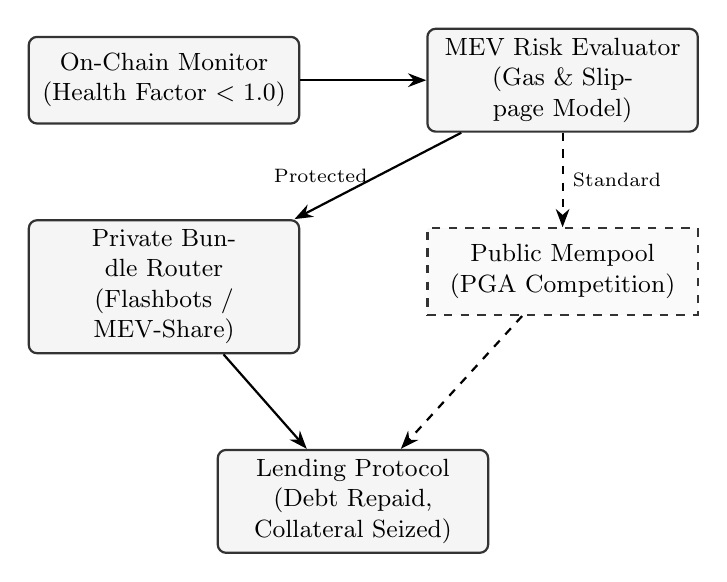
\begin{tikzpicture}[
    node distance=1.2cm and 1.5cm,
    every node/.style={font=\small},
    block/.style={rectangle, draw=black!80, fill=black!4, rounded corners=3pt, text width=3.2cm, minimum height=1.1cm, align=center, line width=0.8pt},
    mempool/.style={rectangle, draw=black!80, dashed, fill=black!2, text width=3.2cm, minimum height=1.1cm, align=center, line width=0.8pt},
    arrow/.style={-{Stealth[scale=1.0]}, line width=0.8pt}
]
% Nodes
\node[block] (monitor) {On-Chain Monitor\\(Health Factor $< 1.0$)};
\node[block, right=1.6cm of monitor] (evaluator) {MEV Risk Evaluator\\(Gas \& Slippage Model)};
\node[block, below=1.2cm of monitor] (private) {Private Bundle Router\\(Flashbots / MEV-Share)};
\node[mempool, below=1.2cm of evaluator] (public) {Public Mempool\\(PGA Competition)};
\node[block, below=1.2cm of private, xshift=2.4cm] (protocol) {Lending Protocol\\(Debt Repaid, Collateral Seized)};

% Paths
\draw[arrow] (monitor) -- (evaluator);
\draw[arrow] (evaluator) -- node[left, font=\scriptsize] {Protected} (private);
\draw[arrow, dashed] (evaluator) -- node[right, font=\scriptsize] {Standard} (public);
\draw[arrow] (private) -- (protocol);
\draw[arrow, dashed] (public) -- (protocol);

\end{tikzpicture}
\caption{Transaction flow comparison between private MEV-aware bundling and standard public mempool liquidations.}
\label{fig:liquidation_pipeline}
\end{figure}

Figure~\ref{fig:liquidation_pipeline} compares standard public mempool execution against our MEV-aware pipeline. By establishing an orderly auction process, Reforge aligns incentives across all three primary stakeholders: borrowers retain more residual equity, protocols prevent bad debt accumulation through deterministic single-transaction settlement, and liquidators earn predictable margins based on execution quality rather than gas expenditure.

\clearpage
% !TEX root = ../main.tex
\chapter{Motivation}


\clearpage
% !TEX root = ../main.tex
\chapter{Objective(s)}
\label{chap:objectives}

\section{Primary Objective}
The primary objective of this project is to design, implement, and empirically validate an end-to-end MEV-aware batch auction mechanism for decentralized lending protocols. The proposed system, named \textbf{Reforge}, replaces latency-sensitive Priority Gas Auctions with an objective economic efficiency metric, selecting winning liquidators by \textbf{Net Economic Value} rather than the magnitude of their gas bribes.

\section{Specific Technical and Research Goals}
To realize the primary objective, the project pursues five specific technical milestones:

\begin{enumerate}
    \item \textbf{Mathematical Formulation of the Scoring Metric:}
    Develop an objective scoring function that quantifies the net economic utility generated by competing liquidation bids:
    \begin{equation}
    \mathrm{NEV} = V_{\mathrm{gross}} - C_{\mathrm{gas}} - C_{\mathrm{slippage}}
    \label{eq:nev_formula}
    \end{equation}
    where $V_{\mathrm{gross}}$ represents the nominal liquidation bonus value, $C_{\mathrm{gas}}$ denotes the actual computational execution cost, and $C_{\mathrm{slippage}}$ accounts for secondary decentralized exchange price impact. Figure~\ref{fig:batch_auction_workflow} illustrates the end-to-end auction workflow.

    \begin{figure}[htbp]
    \centering
    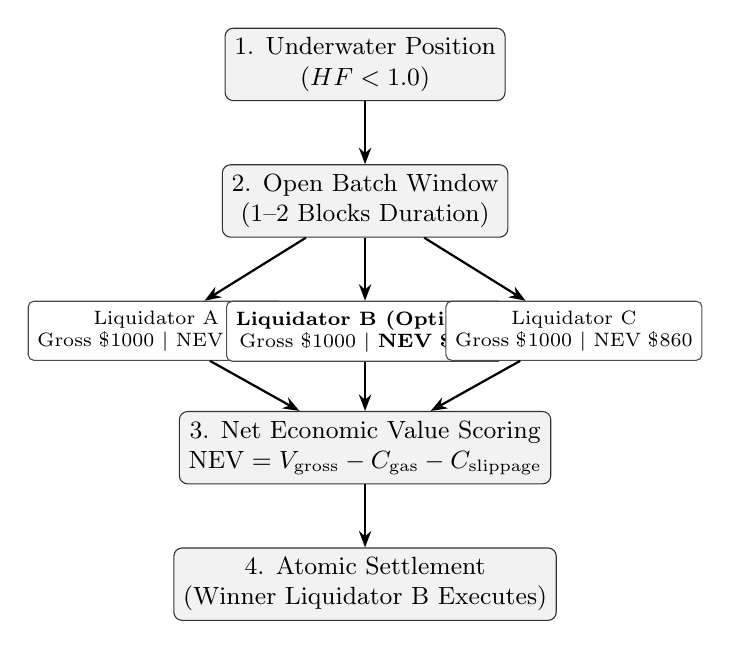
\begin{tikzpicture}[
        node distance=0.9cm and 1.0cm,
        stepnode/.style={rectangle, draw=black!80, fill=black!5, rounded corners=3pt, minimum width=3.4cm, minimum height=0.85cm, align=center, font=\small},
        bidnode/.style={rectangle, draw=black!70, fill=white, rounded corners=2pt, minimum width=3.2cm, minimum height=0.75cm, align=center, font=\scriptsize},
        arrow/.style={-{Stealth[scale=0.9]}, line width=0.8pt}
    ]
    % Main flow nodes
    \node[stepnode] (detect) {1. Underwater Position\\($HF < 1.0$)};
    \node[stepnode, below=0.8cm of detect] (window) {2. Open Batch Window\\(1--2 Blocks Duration)};

    % Competing bids
    \node[bidnode, below left=0.8cm and -0.8cm of window] (b1) {Liquidator A\\Gross \$1000 $\mid$ NEV \$720};
    \node[bidnode, below=0.8cm of window] (b2) {\textbf{Liquidator B (Optimal)}\\Gross \$1000 $\mid$ \textbf{NEV \$900}};
    \node[bidnode, below right=0.8cm and -0.8cm of window] (b3) {Liquidator C\\Gross \$1000 $\mid$ NEV \$860};

    \node[stepnode, below=2.2cm of window] (score) {3. Net Economic Value Scoring\\$\mathrm{NEV} = V_{\mathrm{gross}} - C_{\mathrm{gas}} - C_{\mathrm{slippage}}$};
    \node[stepnode, below=0.8cm of score] (settle) {4. Atomic Settlement\\(Winner Liquidator B Executes)};

    % Arrows
    \draw[arrow] (detect) -- (window);
    \draw[arrow] (window) -- (b1);
    \draw[arrow] (window) -- (b2);
    \draw[arrow] (window) -- (b3);
    \draw[arrow] (b1) -- (score);
    \draw[arrow] (b2) -- (score);
    \draw[arrow] (b3) -- (score);
    \draw[arrow] (score) -- (settle);

    \end{tikzpicture}
    \caption{Reforge batch auction workflow from unhealthy position detection to optimal single-transaction settlement.}
    \label{fig:batch_auction_workflow}
    \end{figure}

    \item \textbf{Smart Contract Architecture Implementation:}
    Design and deploy modular Solidity smart contracts on an EVM-compatible execution environment using Foundry:
    \begin{itemize}
        \item \texttt{LendingPool.sol}: Manages collateral deposits, borrowing accounting, and interest rate accrual.
        \item \texttt{LiquidationAuction.sol}: Coordinates discrete 1--2 block auction windows, registers liquidator commitments, and executes atomic settlements.
        \item \texttt{HealthFactorLib.sol}: Provides optimized, gas-efficient on-chain health factor calculations.
    \end{itemize}

    \item \textbf{Real-Time Asynchronous Backend Infrastructure:}
    Construct a low-latency backend coordinator in Node.js and TypeScript utilizing Fastify, viem, and Redis/BullMQ to subscribe to blockchain block headers, identify unhealthy loan positions ($HF < 1.0$), ingest liquidator bids, and dispatch winning bundles.

    \item \textbf{Web Portal and Liquidator Marketplace:}
    Build a responsive web application using Next.js 16, React 19, and Tailwind CSS to display protocol solvency metrics, real-time liquidation auctions, and an interactive simulation laboratory for researchers.

    \item \textbf{Empirical Simulation and Comparative Evaluation:}
    Construct a Python-based simulation engine to run Monte Carlo market stress tests, comparing Reforge against baseline PGA protocols across key performance indicators: borrower collateral retention, liquidator profit margins, total network gas expenditure, and auction settlement latency.
\end{enumerate}

\section{Tripartite Stakeholder Alignment}
A foundational goal of Reforge is achieving balanced incentives across all three primary DeFi participants, as summarized in Table~\ref{tab:tripartite_alignment}.

\begin{table}[htbp]
\centering
\caption{Incentive alignment comparison between conventional systems and Reforge.}
\label{tab:tripartite_alignment}
\begin{tabular}{p{2.5cm}|p{5.5cm}|p{6.0cm}}
\hline
\textbf{Stakeholder} & \textbf{Conventional System (PGA)} & \textbf{Reforge Batch Auction} \\
\hline
\textbf{Borrower} & Forfeits static 5\%--10\% collateral penalty regardless of market depth. & Retains residual equity by clearing debt at dynamic, competitive discounts. \\
\hline
\textbf{Protocol} & High transaction failure rates during mempool spikes lead to bad debt. & Guaranteed single-transaction execution ensures reliable debt recovery. \\
\hline
\textbf{Liquidator} & Surrenders 70\%--90\% of gross profit to block builders in gas wars. & Captures sustainable profit margins based on routing and DEX efficiency. \\
\hline
\end{tabular}
\end{table}

\clearpage
% !TEX root = ../main.tex
\chapter{Scope of the Project}
\label{chap:scope}

\section{System Architecture and Layer Decomposition}
The scope of the Reforge project spans four interconnected technological tiers, ensuring a comprehensive implementation from core smart contracts to empirical research tooling:

\begin{enumerate}
    \item \textbf{Smart Contract Execution Layer:}
    Implements decentralized financial logic in Solidity ($\ge 0.8.24$) using the Foundry toolchain. The layer manages user balances, computes collateral health factors, enforces the discrete auction lifecycle, and executes flash repayments and collateral payouts atomically.
    
    \item \textbf{Backend Coordination and Event Pipeline:}
    Developed in Node.js and TypeScript using the Fastify framework. It maintains persistent WebSocket connections to the blockchain RPC, detects blocks where positions breach $HF = 1.0$, manages auction state transitions using Redis and BullMQ, and evaluates competing liquidator bids using the Net Economic Value scoring function.
    
    \item \textbf{Frontend User Interface and Telemetry Portal:}
    Built with Next.js 16, React 19, and Tailwind CSS. The interface provides end-users with collateral health dashboards, presents liquidators with a real-time auction marketplace, and offers researchers interactive visualization tools.
    
    \item \textbf{Empirical Research and Simulation Engine:}
    Constructed in Python 3.12 utilizing NumPy, Pandas, and Matplotlib. It simulates synthetic price shocks, replays historical Ethereum market downturns, and benchmarks the economic outcomes of batch auctions against Priority Gas Auctions.
\end{enumerate}

Figure~\ref{fig:system_architecture} illustrates the cross-tier dataflow and interaction among these four operational components.

\begin{figure}[htbp]
\centering
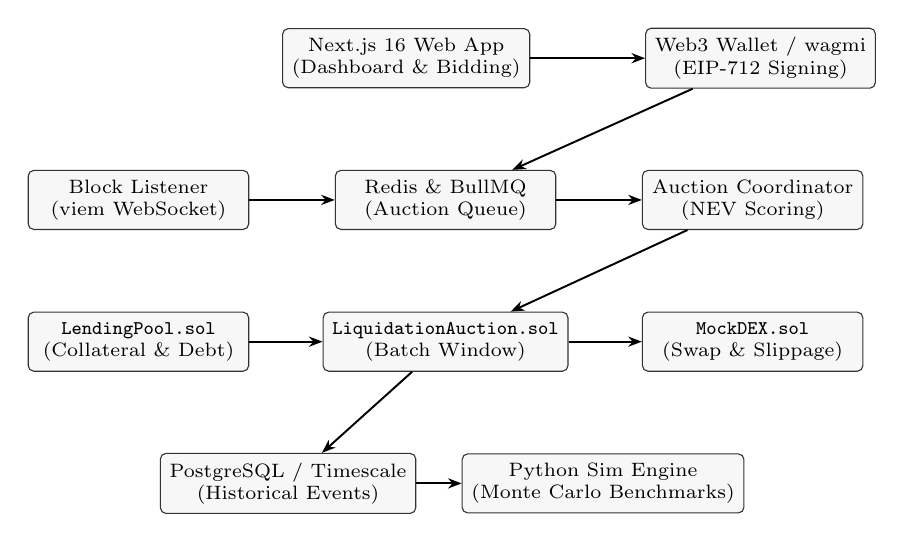
\begin{tikzpicture}[
    node distance=0.8cm and 0.8cm,
    comp/.style={rectangle, draw=black!80, fill=black!3, rounded corners=2pt, minimum width=2.8cm, minimum height=0.75cm, align=center, font=\scriptsize},
    arrow/.style={-{Stealth[scale=0.8]}, line width=0.7pt}
]

% Tier 1: Frontend
\node[comp] (nextjs) at (0, 4.0) {Next.js 16 Web App\\(Dashboard \& Bidding)};
\node[comp] (wallet) at (4.5, 4.0) {Web3 Wallet / wagmi\\(EIP-712 Signing)};

% Tier 2: Backend
\node[comp] (listener) at (-3.4, 2.2) {Block Listener\\(viem WebSocket)};
\node[comp] (queue) at (0.5, 2.2) {Redis \& BullMQ\\(Auction Queue)};
\node[comp] (engine) at (4.4, 2.2) {Auction Coordinator\\(NEV Scoring)};

% Tier 3: Contracts
\node[comp] (pool) at (-3.4, 0.4) {\texttt{LendingPool.sol}\\(Collateral \& Debt)};
\node[comp] (auction) at (0.5, 0.4) {\texttt{LiquidationAuction.sol}\\(Batch Window)};
\node[comp] (dex) at (4.4, 0.4) {\texttt{MockDEX.sol}\\(Swap \& Slippage)};

% Tier 4: Research
\node[comp] (db) at (-1.5, -1.4) {PostgreSQL / Timescale\\(Historical Events)};
\node[comp] (sim) at (2.5, -1.4) {Python Sim Engine\\(Monte Carlo Benchmarks)};

% Connections
\draw[arrow] (nextjs) -- (wallet);
\draw[arrow] (wallet) -- (queue);
\draw[arrow] (listener) -- (queue);
\draw[arrow] (queue) -- (engine);
\draw[arrow] (engine) -- (auction);
\draw[arrow] (pool) -- (auction);
\draw[arrow] (auction) -- (dex);
\draw[arrow] (auction) -- (db);
\draw[arrow] (db) -- (sim);

\end{tikzpicture}
\caption{End-to-end multi-tier system architecture of the Reforge liquidation platform.}
\label{fig:system_architecture}
\end{figure}

\section{Operational Assumptions and Boundaries}
To maintain a well-defined project scope, Reforge operates under specific foundational parameters:
\begin{itemize}
    \item \textbf{Target Blockchain Environment:} The protocol is designed for Ethereum Mainnet and EVM-compatible Layer-2 rollups (such as Arbitrum and Optimism) that maintain deterministic block execution.
    \item \textbf{Oracle Architecture:} Asset valuations rely on external decentralized price oracles (such as Chainlink) with standard heartbeat and deviation update thresholds.
    \item \textbf{Auction Window Duration:} The discrete batch auction window is bounded between 1 and 2 blocks (approximately 12 to 24 seconds on Ethereum L1). This duration balances adequate liquidator participation against the risk of rapid price depreciation.
\end{itemize}

\section{The Latency vs. Solvency Trade-off}
A central analytical challenge within the project scope is evaluating the \textbf{Auction Latency Problem}. In conventional protocols, liquidation is continuous and instantaneous: the first transaction submitted in the next block clears the loan. Reforge introduces an explicit time window of 1--2 blocks to collect and score competing bids.

During this brief window, if the collateral price experiences an extreme flash crash, the position could deteriorate into negative equity (where debt value exceeds total collateral value) before settlement occurs. Quantifying this exact trade-off---whether the massive reduction in MEV gas waste and preserved borrower equity outweighs the marginal risk of auction latency---constitutes a core focus of our research simulation.

\section{Out-of-Scope Boundaries}
The following aspects are explicitly excluded from the current project scope:
\begin{itemize}
    \item \textbf{Cross-Chain Atomic Settlement:} Multi-chain liquidations spanning distinct consensus layers via bridges are excluded; all settlement occurs natively on a single EVM state machine.
    \item \textbf{Under-Collateralized Lending:} The system focuses exclusively on overcollateralized lending pools; identity-based credit scoring or zero-collateral lending is out of scope.
    \item \textbf{Proprietary Off-Chain Bot Strategies:} The project specifies the protocol-level scoring mechanism and reference liquidator interfaces, but does not encompass proprietary high-frequency trading arbitrage algorithms.
\end{itemize}

\clearpage
% !TEX root = ../main.tex
\chapter{Related Work}
\label{chap:related_work}

The design and evaluation of Reforge builds directly upon recent academic breakthroughs spanning DeFi liquidation mechanics, Maximal Extractable Value (MEV), Proposer-Builder Separation (PBS), and consensus-level order-fairness.

\section{Empirical Studies on DeFi Liquidations}
A critical pillar of lending protocol stability is understanding how liquidation mechanisms behave under real market stress:

\begin{itemize}
    \item \textbf{Qin et al. (IMC 2021):} Conducted the first large-scale empirical evaluation of liquidations across Aave, Compound, MakerDAO, and dYdX~\cite{qin2021empirical}. The authors demonstrated that static liquidation discounts (5\%--10\%) transfer oversized economic surplus from distressed borrowers to liquidators. Even in highly liquid market environments with minimal execution frictions, borrowers were forced to forfeit the full fixed penalty. Furthermore, they proved that liquidators strategically optimize partial repayments and gas bids to maximize extraction.
    
    \item \textbf{Tian and Xu (Bank of Canada 2025):} Provided direct empirical comparison between fixed-spread models (Aave) and competitive Dutch auctions (MakerDAO)~\cite{tian2025liquidation}. Their findings reveal that competitive auctions reduce average liquidation discounts from 5.0\% to 1.8\% (a 64\% reduction) and cut secondary market price impact by 81\% (from 0.054\% to 0.010\%). Their analysis highlights two competing economic forces: the \textit{participation effect} (auctions attract more diverse searchers) and the \textit{competition effect} (bidding drives clearance prices closer to fair market value).
\end{itemize}

\section{MEV Foundations and Priority Gas Auctions}
The theoretical and empirical understanding of transaction reordering in transparent mempools is rooted in seminal MEV research:

\begin{itemize}
    \item \textbf{Daian et al. (Flash Boys 2.0, IEEE S\&P 2019):} First formalized Maximal Extractable Value and demonstrated that pending transactions in public mempools invite automated Priority Gas Auctions (PGAs)~\cite{daian2019flashboys}. The authors proved that when extractable value is large relative to block subsidies, rational miners are economically incentivized to execute ``time-bandit attacks''---reorganizing historical blocks to steal past MEV opportunities.
    
    \item \textbf{Qin et al. (Quantifying BEV, IEEE S\&P 2022):} Measured over \$540.54 million in extracted MEV across 32 months of Ethereum mainnet data~\cite{qin2022quantifying}. The study demonstrated that liquidations constitute 26\% of all extracted value (second only to DEX arbitrage), with single liquidation events yielding profits up to \$4.1 million.
\end{itemize}

\section{Proposer-Builder Separation and Private Flow}
With the introduction of MEV-Boost following Ethereum's transition to Proof-of-Stake, the structural dynamics of MEV shifted into specialized builder auctions:

\begin{itemize}
    \item \textbf{Pai and Resnick (2023):} Analyzed the structural advantages enjoyed by vertically integrated searcher-builders in MEV-Boost auctions~\cite{pai2023integrated}. They proved that integrated builders observe competing bundles with zero external communication latency and effectively participate in second-price auction dynamics, while independent liquidators face the ``winner's curse''.
    
    \item \textbf{Wang et al. (2024):} Empirically measured private order flow dynamics on Ethereum, demonstrating that the top three block builders construct over 95\% of all blocks~\cite{wang2024private}. This market concentration proves that private builder channels do not eliminate unfair competition, but rather centralize it.
    
    \item \textbf{Natale and Moser (2023):} Investigated artificial latency games in PBS, showing that block proposers systematically delay block proposals by 500--1000ms to extract a median 1.28\% increase in MEV bribes~\cite{natale2023artificial}.
\end{itemize}

Figure~\ref{fig:pbs_supply_chain} illustrates the modern MEV supply chain operating between searchers, block builders, and consensus validators under PBS.

\begin{figure}[htbp]
\centering
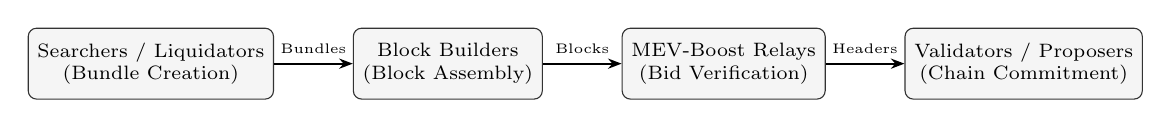
\begin{tikzpicture}[
    node distance=1.2cm,
    stage/.style={rectangle, draw=black!80, fill=black!4, rounded corners=3pt, minimum width=2.4cm, minimum height=0.9cm, align=center, font=\scriptsize},
    arrow/.style={-{Stealth[scale=0.8]}, line width=0.7pt}
]
\node[stage] (searchers) {Searchers / Liquidators\\(Bundle Creation)};
\node[stage, right=1.0cm of searchers] (builders) {Block Builders\\(Block Assembly)};
\node[stage, right=1.0cm of builders] (relays) {MEV-Boost Relays\\(Bid Verification)};
\node[stage, right=1.0cm of relays] (validators) {Validators / Proposers\\(Chain Commitment)};

\draw[arrow] (searchers) -- node[above, font=\tiny] {Bundles} (builders);
\draw[arrow] (builders) -- node[above, font=\tiny] {Blocks} (relays);
\draw[arrow] (relays) -- node[above, font=\tiny] {Headers} (validators);

\end{tikzpicture}
\caption{The modern MEV supply chain under Proposer-Builder Separation (PBS).}
\label{fig:pbs_supply_chain}
\end{figure}

\section{Order-Fairness and Security Taxonomies}
\begin{itemize}
    \item \textbf{Kelkar et al. (CRYPTO 2020):} Introduced the concept of \textit{order-fairness} for Byzantine consensus protocols (the Aequitas family)~\cite{kelkar2020order}, proving that standard consensus safety and liveness guarantees do not protect against sequence manipulation by block proposers.
    
    \item \textbf{Eskandari et al. (FC 2019):} Formulated the canonical front-running taxonomy: displacement, insertion, and suppression~\cite{eskandari2019sok}. Standard mempool liquidation races represent pure displacement attacks, where searchers copy and outbid competitors.
    
    \item \textbf{Werner et al. (2021) and Gogol et al. (2024):} Systematized DeFi risk frameworks~\cite{werner2021sok,gogol2024sok}, demonstrating that lending protocol insolvency arises from external economic incentive failures and mempool latency games rather than smart contract coding bugs.
\end{itemize}

\section{Comparative Synthesis Matrix}
Table~\ref{tab:lit_comparison} synthesizes how Reforge compares against prevailing liquidation architectures in decentralized finance.

\begin{table}[htbp]
\centering
\small
\caption{Architectural comparison of liquidation mechanisms across DeFi protocols.}
\label{tab:lit_comparison}
\begin{tabular}{p{2.2cm}|p{3.0cm}|p{3.0cm}|p{3.2cm}|p{2.2cm}}
\hline
\textbf{Protocol} & \textbf{Mechanism Type} & \textbf{Pricing Model} & \textbf{MEV Resistance} & \textbf{Borrower Equity} \\
\hline
Aave v3 & First-come Mempool & Fixed Penalty (5--10\%) & None (PGA Gas Wars) & Low (Static Loss) \\
Compound v3 & First-come Mempool & Fixed Penalty (5--8\%) & None (PGA Gas Wars) & Low (Static Loss) \\
MakerDAO & Dutch Auction & Descending Price Curve & Moderate (Latency Bidding) & Medium (Dynamic) \\
\textbf{Reforge} & \textbf{Batch Auction} & \textbf{Net Economic Value} & \textbf{High (Order-Fair)} & \textbf{High (Maximized)} \\
\hline
\end{tabular}
\end{table}

\section{Conclusion}
The literature confirms that while conventional liquidation systems successfully maintain protocol solvency during benign market conditions, their reliance on first-come public mempool races imposes severe costs: excessive borrower collateral loss, catastrophic gas wars, and block-builder centralization. Existing auction designs, while superior to fixed spreads, remain susceptible to latency exploitation and builder monopolies. This establishes a clear need for Reforge's application-level batch clearing mechanism.

\section{Future Scope}
Future extensions of this work include integrating zero-knowledge proofs (ZKPs) for private bid commitments, extending the batch clearing model to cross-chain lending protocols via LayerZero or Chainlink CCIP, and applying reinforcement learning algorithms to dynamically adjust the discrete auction window duration in response to real-time market volatility.

\clearpage
% !TEX root = ../main.tex
\chapter{HARDWARE \& SOFTWARE REQUIREMENTS}

\clearpage
% !TEX root = ../main.tex
\chapter{Predicted Timeline for the Project}
\label{chap:timeline}

The implementation and scientific evaluation of Reforge are structured across an eight-month academic timeline, partitioned into six distinct engineering and research phases.

\section{Phase Breakdown and Sprint Structure}
The project employs an iterative development methodology with bi-weekly development sprints to ensure continuous integration, testing, and empirical feedback:

\begin{itemize}
    \item \textbf{Phase 1: Literature Review \& Mathematical Modeling (Months 1--2):}
    Comprehensive synthesis of academic literature on MEV, Proposer-Builder Separation, and DeFi liquidation mechanisms. Formal derivation and parameter tuning of the Net Economic Value (NEV) scoring equation.
    
    \item \textbf{Phase 2: Smart Contract Core Development (Months 3--4):}
    Implementation of the core Solidity contracts (\texttt{LendingPool.sol}, \texttt{LiquidationAuction.sol}, \texttt{HealthFactorLib.sol}). Writing automated unit tests, fuzz testing suites, and invariant checks in Foundry.
    
    \item \textbf{Phase 3: Real-Time Backend Coordination Pipeline (Months 4--5):}
    Constructing the Node.js/TypeScript backend services, including WebSocket RPC block subscription, Redis/BullMQ opportunity scheduling, and the off-chain bid ingestion and scoring coordinator.
    
    \item \textbf{Phase 4: Frontend Web Portal \& Marketplace Terminal (Months 5--6):}
    Developing the Next.js 16 user interface, integrating wallet connection hooks via wagmi/viem, rendering live liquidation auctions, and building the interactive research telemetry console.
    
    \item \textbf{Phase 5: Empirical Simulation \& Benchmark Experiments (Months 6--7):}
    Constructing the Python-based Monte Carlo market simulation engine. Running stress tests under historical market shock conditions (e.g., March 2020 Black Thursday, May 2022 Terra-Luna collapse) to evaluate collateral retention and latency trade-offs against baseline PGA mechanisms.
    
    \item \textbf{Phase 6: Analysis, Documentation \& Thesis Compilation (Months 7--8):}
    Synthesizing simulation results, drafting academic research papers, completing formal thesis documentation, and preparing the final project defense presentation.
\end{itemize}

\section{Milestone Schedule}
Table~\ref{tab:project_milestones} details the projected milestone deliverables across each phase.

\begin{table}[htbp]
\centering
\caption{Detailed project milestones and timeline schedule.}
\label{tab:project_milestones}
\begin{tabular}{c|p{4.5cm}|c|p{6.0cm}}
\hline
\textbf{Phase} & \textbf{Milestone Task} & \textbf{Timeline} & \textbf{Key Deliverable} \\
\hline
\textbf{1} & Literature Survey \& NEV Formulation & Month 1--2 & Literature review synthesis and formal scoring specification. \\
\hline
\textbf{2} & Smart Contract Implementation & Month 3--4 & Foundry test suite with $>$95\% code coverage and invariant tests. \\
\hline
\textbf{3} & Real-Time Backend Engine & Month 4--5 & Functional WebSocket listener and Redis queue scoring service. \\
\hline
\textbf{4} & Next.js Web Interface & Month 5--6 & Live protocol dashboard, auction terminal, and telemetry UI. \\
\hline
\textbf{5} & Empirical Simulation & Month 6--7 & Monte Carlo experimental benchmark dataset and comparative plots. \\
\hline
\textbf{6} & Documentation \& Defense & Month 7--8 & Final B.Tech project synopsis, thesis dissertation, and defense slides. \\
\hline
\end{tabular}
\end{table}

\clearpage
% !TEX root = ../main.tex
\chapter{Conclusion}
\label{chap:conclusion}

Decentralized lending protocols are foundational building blocks of the decentralized financial ecosystem, yet their reliance on first-come, first-served liquidations in public mempools has introduced severe systemic vulnerabilities. As demonstrated by recent empirical literature, Priority Gas Auctions cause 70\% to 90\% of gross liquidation profits to leak to consensus block builders, force distressed borrowers to forfeit excessive collateral via static penalty rates, and exacerbate secondary market price slippage through uncoordinated collateral dumping.

This project introduces \textbf{Reforge}, an end-to-end MEV-aware batch auction liquidation mechanism designed to replace predatory gas-bidding races with objective economic efficiency. By accumulating competing liquidator bids across a discrete, short auction window (1--2 blocks) and evaluating bids via the \textbf{Net Economic Value} metric:
\begin{equation}
\mathrm{NEV} = V_{\mathrm{gross}} - C_{\mathrm{gas}} - C_{\mathrm{slippage}}
\end{equation}
Reforge ensures that liquidations are awarded to participants who execute with the lowest transaction overhead and minimal secondary market price impact.

The system is comprehensively architected across four modular tiers:
\begin{enumerate}
    \item \textbf{EVM Smart Contracts:} Delivering robust collateral custody, lending pools, discrete auction lifecycles, and atomic settlement routines implemented in Solidity.
    \item \textbf{High-Performance Backend Pipeline:} Providing real-time WebSocket block listening, asynchronous job queue scheduling via Redis/BullMQ, and off-chain bid ingestion and scoring.
    \item \textbf{User and Liquidator Portal:} Offering a modern Next.js 16 web interface for protocol health telemetry and liquidator auction participation.
    \item \textbf{Empirical Simulation Engine:} Enabling reproducible Monte Carlo benchmarking across historical crash regimes to quantify the precise trade-off between auction latency and protocol solvency.
\end{enumerate}

By aligning the economic incentives of borrowers, protocols, and liquidators, Reforge demonstrates that application-level mechanism redesign can successfully mitigate MEV extraction. The project provides an open-source, academically grounded blueprint for building more resilient, fair, and capital-efficient lending architectures in decentralized finance.

\clearpage
% !TEX root = ../main.tex
\chapter*{References}

\clearpage
\appendix
% !TEX root = ../main.tex
\chapter{Plagiarism Report}
\section{Plagiarism Report}
\section{AI Content Report}


\end{document}

